
\documentclass[a4paper,oneside,10pt]{article}
\usepackage[utf8]{inputenc}
\usepackage[T1]{fontenc} 
\usepackage{amsmath,amssymb}
\usepackage{fullpage}
\usepackage{graphicx}
\usepackage{url}
\usepackage{xspace}
\usepackage[french]{babel}
\usepackage{multicol}
\usepackage{geometry}
\usepackage{float}
\geometry{hmargin=2cm,vmargin=1.8cm}
\title{Projet ACVL - Rapport}

\author{DANTIGNY Raynald, DE GEA Jordan, DUCLOT William, RABOURG Simon}

\begin{document}

\maketitle

\section{Analyse}
\subsection{Diagramme de classes d'analyse}
A MODIFIER pour résumé/parties
\begin{figure}[H]
\begin{center}
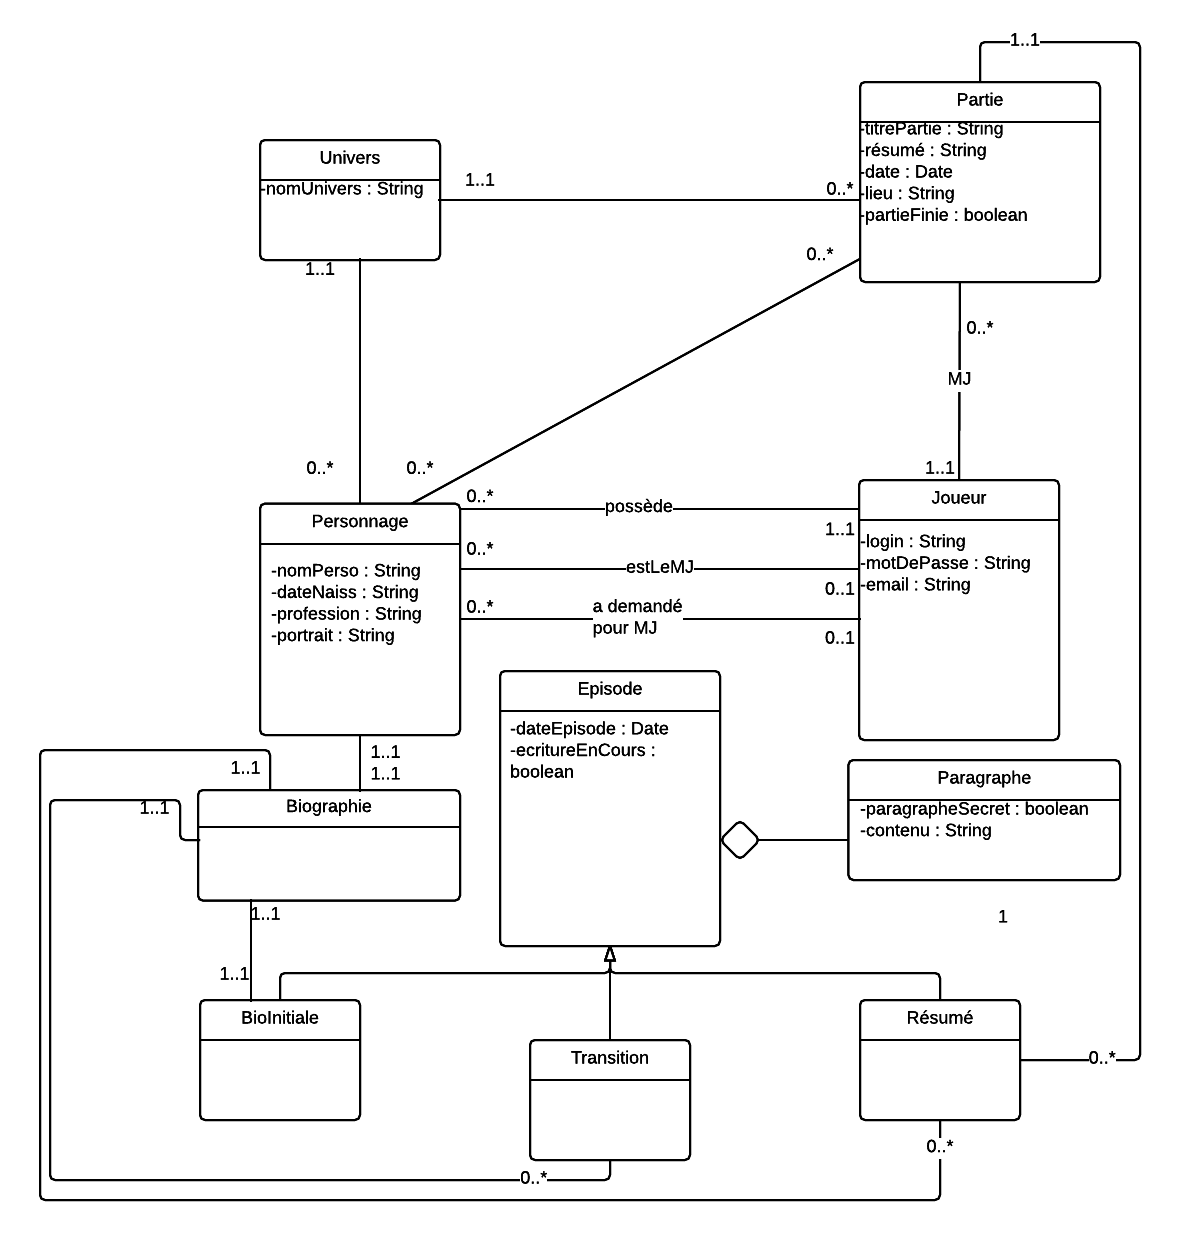
\includegraphics[width=10cm]{images/classe/DiagrammeClasse.png} 
	\caption{Diagramme de classes d'analyse}
\end{center}
\end{figure}
\subsection{Cas d'utilisation}
\begin{figure}[H]
	\begin{center}
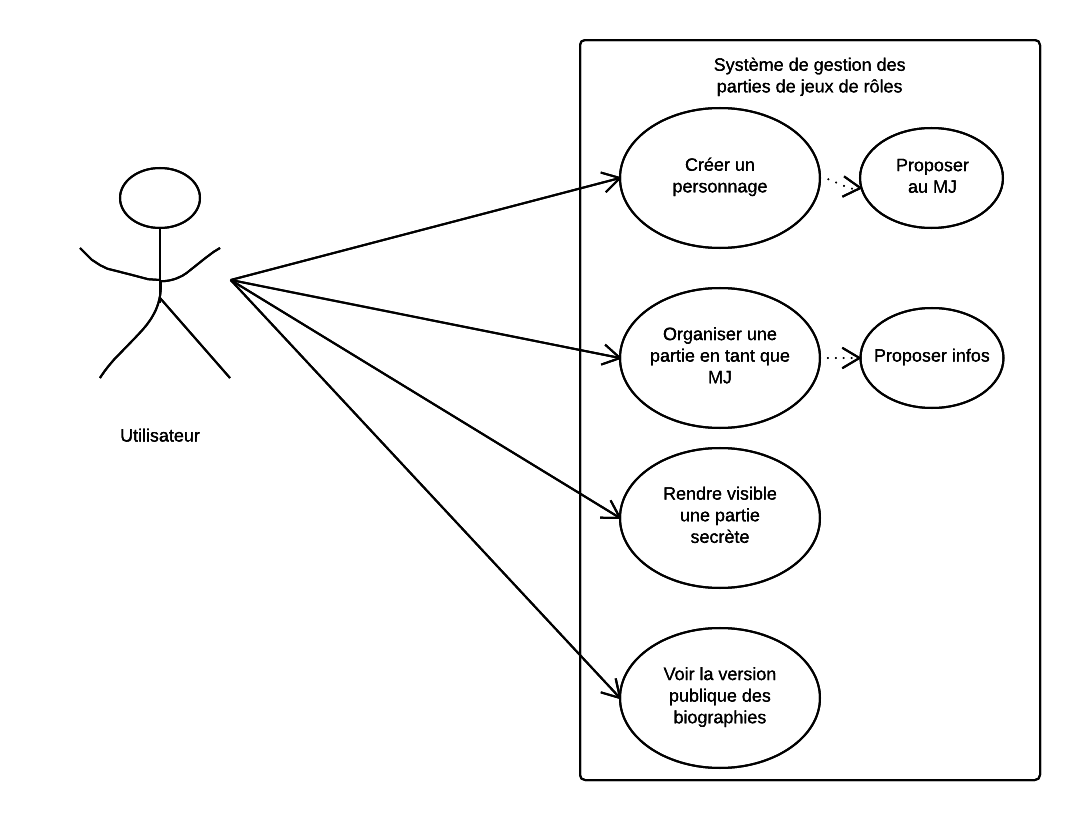
\includegraphics[width=10cm]{images/utilisation/UserCU.png} 
	\caption{Cas d'utilisation pour l'utilisateur}
\end{center}
\end{figure}

\begin{figure}[H]
	\begin{center}
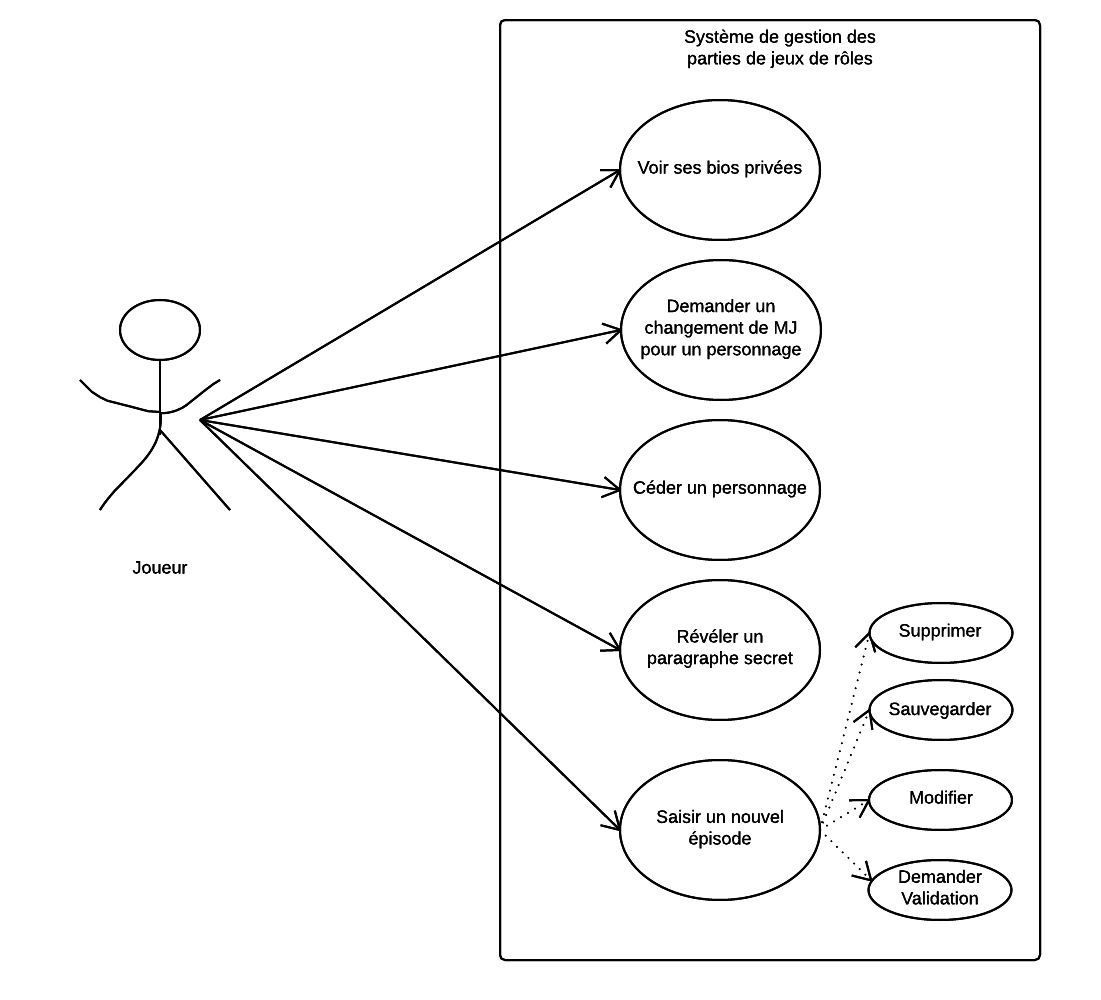
\includegraphics[width=10cm]{images/utilisation/JoueurCU.png}
	\caption{Cas d'utilisation pour le joueur}
\end{center}
\end{figure}
\begin{figure}[H]
	\begin{center}
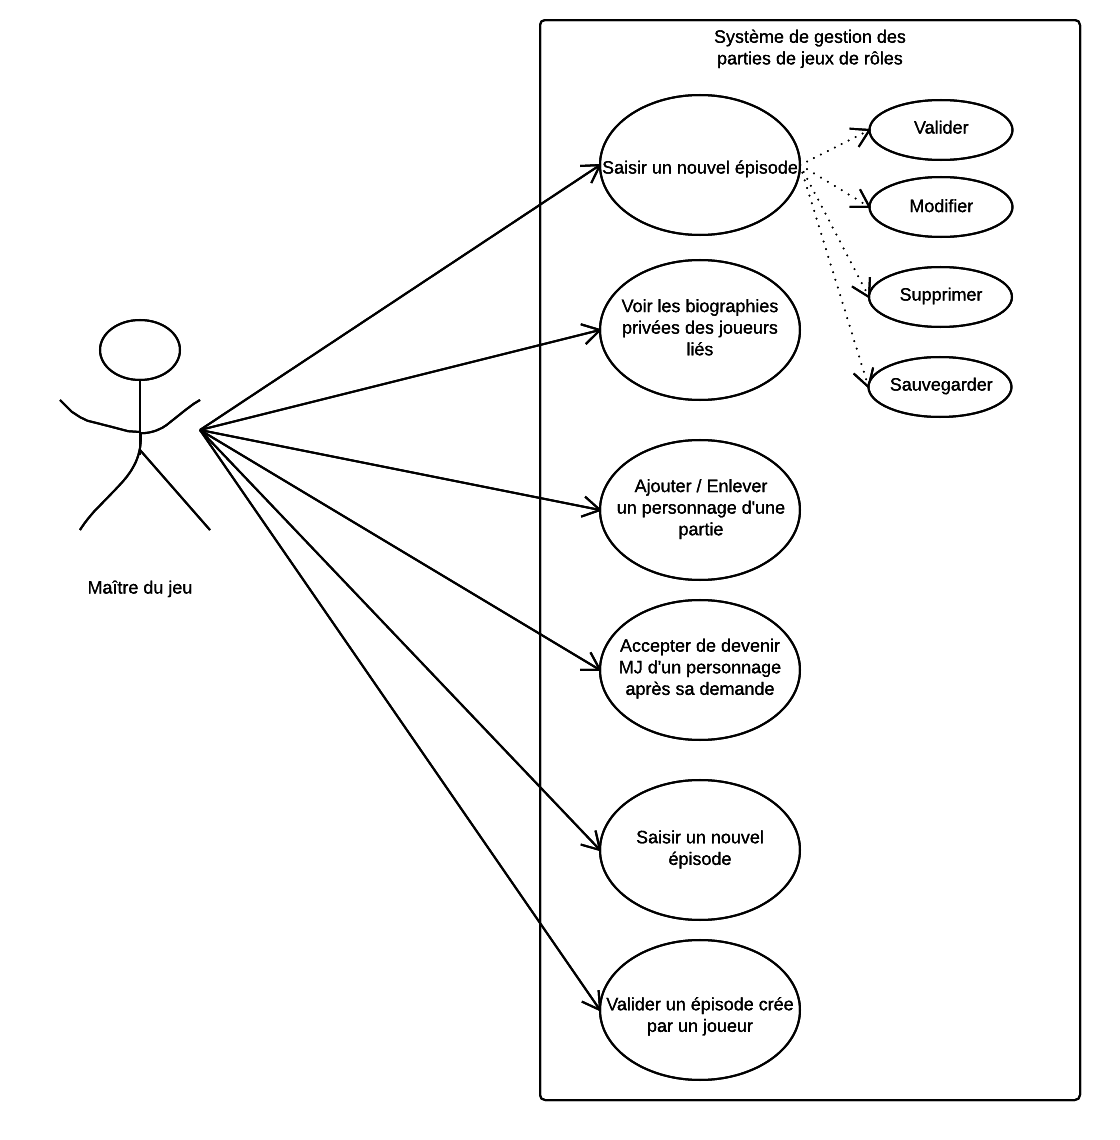
\includegraphics[width=10cm]{images/utilisation/MJCU.png}  
	\caption{Cas d'utilisation pour le Maitre du Jeu}
\end{center}
\end{figure}

\subsection{Diagrammes de séquence système}
\begin{figure}[H]
	\begin{center}
		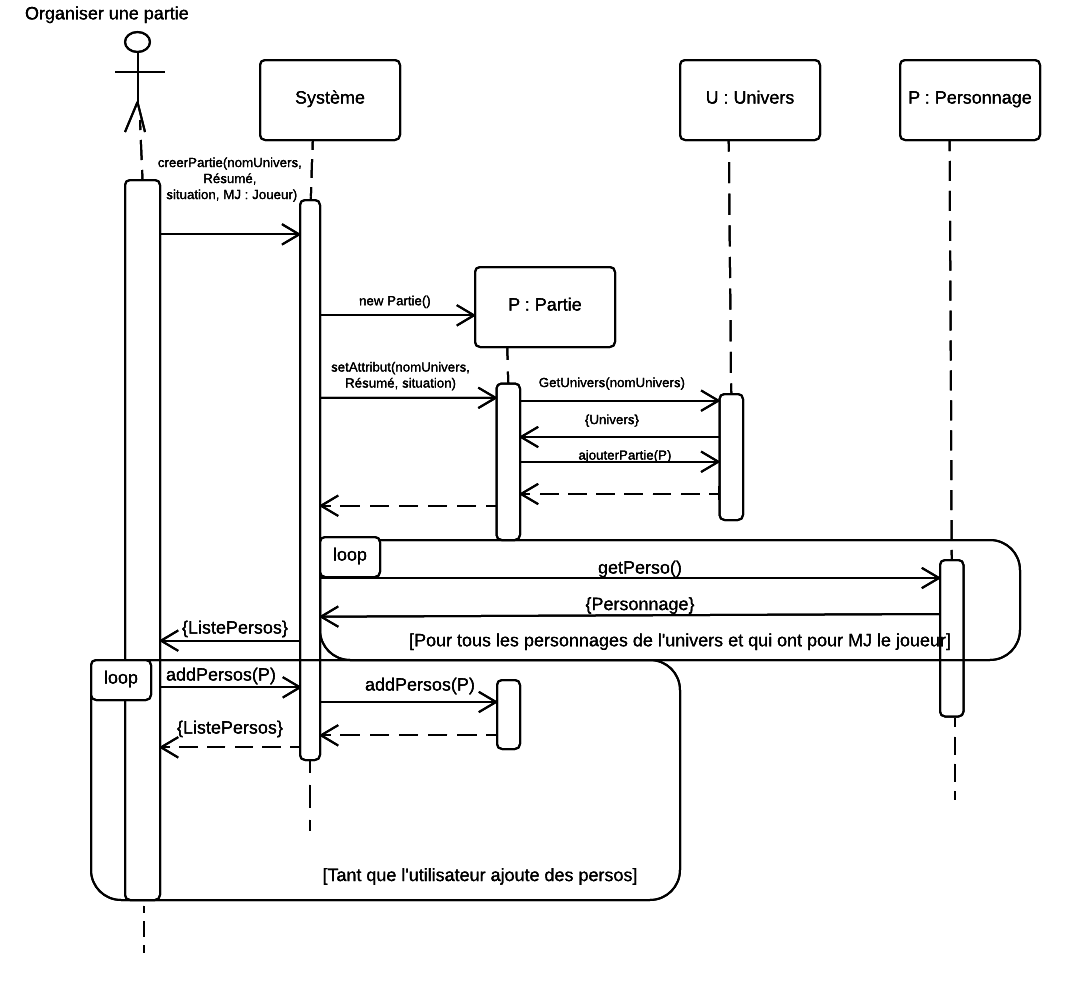
\includegraphics[width=10cm]{images/sequence/DS-OrganiserPartie.png}  
		\caption{Organiser une partie}
	\end{center}
\end{figure}
\begin{figure}[H]
	\begin{center}
		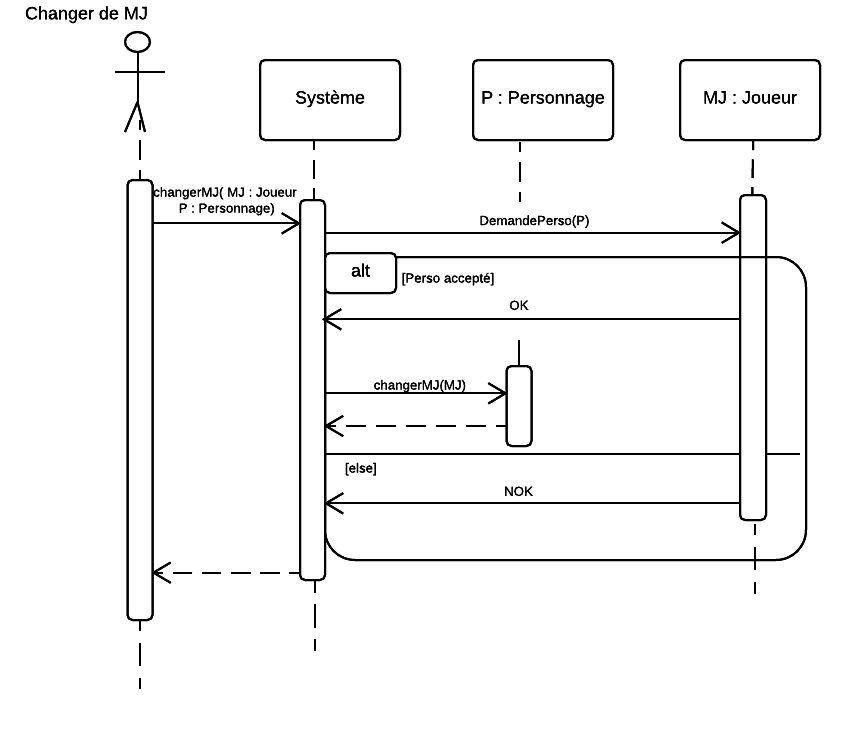
\includegraphics[width=10cm]{images/sequence/DS-ChangerMJ.png}  
		\caption{Changer de maître du jeu pour un personnage}
	\end{center}
\end{figure}
\begin{figure}[H]
	\begin{center}
		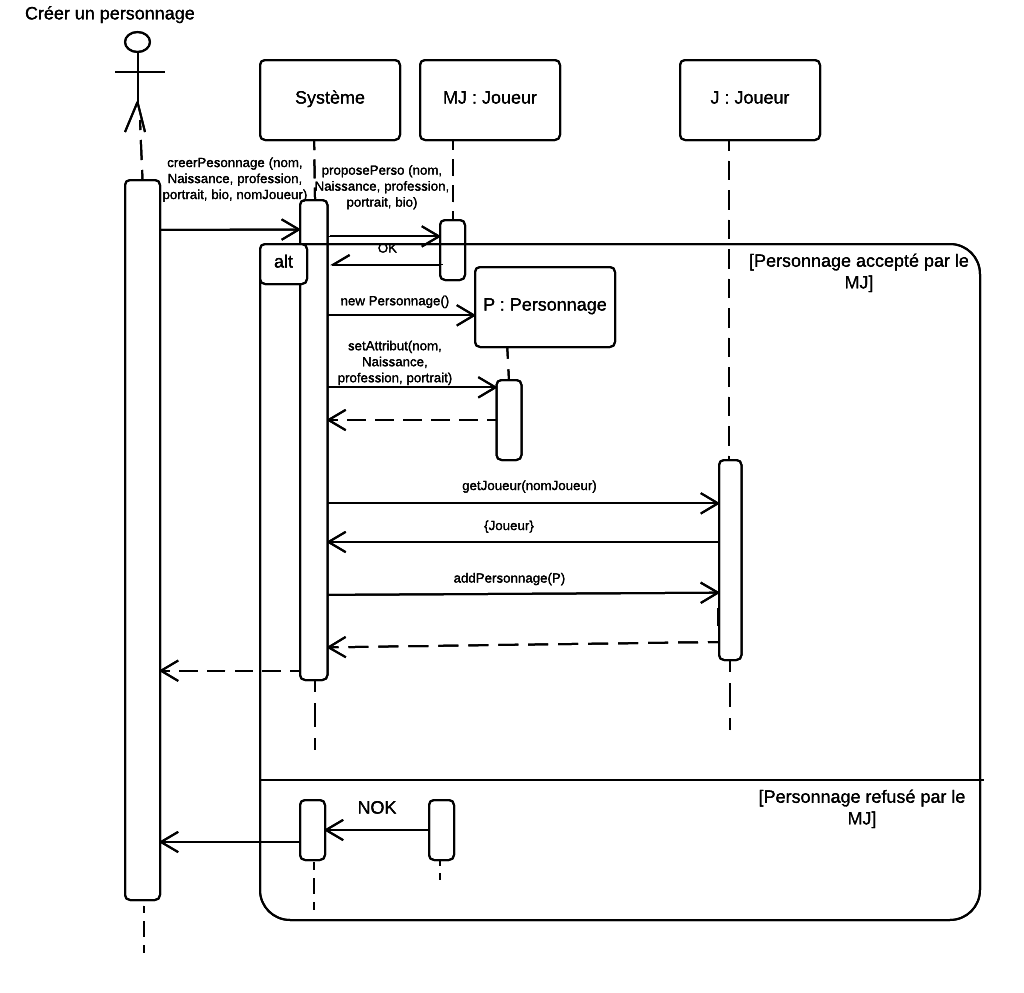
\includegraphics[width=10cm]{images/sequence/DS-CreerPerso.png}  
		\caption{Créer un personnage}
	\end{center}
\end{figure}
\section{Conception}
\subsection{Diagramme d'architecture MVC}
\subsection{Diagramme de classe logiciel}

\subsection{Diagrammes d'Etats-transitions}
Ici diagramme sur ET sur les transfert de compte (Simon).


\section{Manuel Utilisateur}


\section{Bilan}


\end{document}
